% =====================================================================
%  VISTA — appendix sections updated for all SEVEN models
%  (Gemma 4 31B, Qwen 2.5 32B, LLaMA 3.1 8B, Claude Haiku 4.5,
%   GPT-4.1-mini, GPT-5-mini, Claude Sonnet 5)
%
%  Drop-in replacements for the corresponding \section blocks in your
%  working copy. Each block below replaces one whole \section{...},
%  from the \section line through to just before the next \section.
%
%  Appendix sections NOT listed here need no change: Schwartz Value
%  Profile Enumeration, Human Pilot Per-Cell Decision Shift, Qualitative
%  Examples, Lambda Sweep, Dataset & Prompt Templates, Human Study
%  Value Trade-offs. They contain no per-model numbers.
%
%  NOTE ON SECTION TITLES: your copy titles block D "Paraphrase Noise
%  Study:" — keep your title, only the body below changed.
% =====================================================================


% --------------------------------------------------------------------
% A. Full Per-Axis Logistic Regression Coefficients
% --------------------------------------------------------------------
\section{Full Per-Axis Logistic Regression Coefficients}
\label{app:lr}

\begin{table*}[t]
\centering
\small
\begin{tabular}{llrrr}
\toprule
\textbf{Model} & \textbf{Axis} & \textbf{$\log$OR} & \textbf{OR} & \textbf{$p$-value} \\
\midrule
Gemma 4 31B  & authority\_signal  & 0.565 & 1.76 & $<10^{-7}$ \\
             & self\_preservation & 0.495 & 1.64 & $<10^{-6}$ \\
\addlinespace
Qwen 2.5 32B & self\_preservation & 0.417 & 1.52 & $<10^{-3}$ \\
             & authority\_signal  & 0.275 & 1.32 & 0.015 \\
\addlinespace
LLaMA 3.1 8B & self\_preservation & 0.723 & 2.06 & 0.014 \\
             & authority\_signal  & 0.723 & 2.06 & 0.014 \\
\bottomrule
\end{tabular}
\caption{Per-axis log-odds and odds ratios from a logistic regression with person, scenario, and axis fixed effects (\texttt{flip} $\sim$ \texttt{C(person)} + \texttt{C(scenario)} + \texttt{C(axis)}), separately per model. The two top-ranked axes by significance are shown. \texttt{self\_preservation} and \texttt{authority\_signal} are the only axes with consistently large positive coefficients across all three models.}
\label{tab:lr}
\end{table*}

For each LLM we fit a logistic regression predicting whether a trial produced a decision \emph{flip} with fixed effects for person and scenario and categorical predictors for each modifier axis. Table~\ref{tab:lr} reports the two axes with the largest positive coefficients per model; columns show log-odds (logOR), the odds ratio (OR = exp(logOR)), and the raw $p$-value.

\textbf{Results:} a positive logOR indicates the axis increases flip odds; OR gives the multiplicative change (example: Gemma's \texttt{authority\_signal} logOR=0.565 $\rightarrow$ OR$\approx$1.76, i.e., $\approx$76\% higher odds of flipping when an authority cue is present). Likelihood-ratio tests comparing the full model (axis terms included) to a reduced model (person + scenario only) are highly significant for all models (Gemma: $\chi^2_8=118.74$, $p\approx6\times10^{-22}$; Qwen: $\chi^2_8=75.28$, $p\approx4.3\times10^{-13}$; LLaMA: $\chi^2_8=30.70$, $p\approx1.6\times10^{-4}$), indicating axis predictors add explanatory power.

\textbf{Interpretation and reporting:} reported effects are moderate (ORs $\approx$1.3--2.1) --- modifiers substantially increase flip odds but do not deterministically produce flips.

\textbf{A second test covering every model.} The fixed-effects fit above needs per-person terms and was run on the three locally hosted models. We therefore also report the paired McNemar exact test on the same baseline-versus-modifier cells, which needs no such term and so applies uniformly to all seven models (Table~\ref{tab:mcnemar-all}); $p$-values are BH-FDR corrected over the eight axes within each model. Across the 56 (model, axis) tests, 31 are significant at BH-FDR $<0.05$.

\begin{table}[t]
\centering
\footnotesize
\setlength{\tabcolsep}{4pt}
\resizebox{\columnwidth}{!}{%
\begin{tabular}{lrrrr}
\toprule
\textbf{Model} & \textbf{self\_pres.} & \textbf{authority} & \textbf{diffused} & \textbf{\#sig/8} \\
\midrule
Gemma 4 31B  & 7.67$^{***}$ & 5.04$^{***}$ & 0.27$^{***}$ & 5 \\
Qwen 2.5 32B & 3.36$^{***}$ & 2.87$^{***}$ & 0.20$^{***}$ & 8 \\
LLaMA 3.1 8B & 4.40$^{**}$  & 3.43$^{**}$  & 0.62         & 2 \\
Haiku 4.5$^\ddagger$    & 8.20$^{***}$ & 2.00$^{***}$ & 0.42$^{***}$ & 5 \\
GPT-4.1-mini$^\ddagger$ & 3.36$^{***}$ & 2.38$^{***}$ & 0.87         & 3 \\
GPT-5-mini$^\ddagger$   & 3.29$^{***}$ & 1.86$^{**}$  & 0.46$^{**}$  & 4 \\
Sonnet 5$^\ddagger$     & 3.05$^{***}$ & 2.56$^{***}$ & 0.34$^{***}$ & 4 \\
\bottomrule
\end{tabular}}
\caption{McNemar exact-test odds ratios on paired baseline-vs-modifier decisions ($n=950$ pairs per cell), for the two dominant axes and for \texttt{diffused\_responsibility}. $^{***}p<0.001$, $^{**}p<0.01$ after BH-FDR over the eight axes within each model; $\ddagger$ marks models served through provider APIs. \texttt{self\_preservation} and \texttt{authority\_signal} are the two largest positive ORs in every model; \texttt{diffused\_responsibility} is below 1 in every model, i.e.\ it shifts decisions \emph{away} from the modified framing.}
\label{tab:mcnemar-all}
\end{table}


% --------------------------------------------------------------------
% B. Profile-Strength Breakdown  (two tables + text)
% --------------------------------------------------------------------
\section{Profile-Strength Breakdown}
\label{app:strength}

\begin{table}[t]
\centering\footnotesize
\setlength{\tabcolsep}{3.5pt}
\resizebox{\columnwidth}{!}{%
\begin{tabular}{lrrrrrrrr}
\toprule
\textbf{Str} & \textbf{N} & \textbf{Gemma} & \textbf{Qwen} & \textbf{LLaMA} & \textbf{Haiku} & \textbf{GPT4.1} & \textbf{GPT5} & \textbf{Sonnet} \\
\midrule
0  &    80  & 11.25 &  3.75 & 5.00 & 20.00 &  6.25 & 12.50 & 26.25 \\
1  &   400  &  4.75 &  5.25 & 6.50 &  3.75 &  8.25 &  4.75 &  4.00 \\
2  &   800  &  9.38 &  5.75 & 2.50 &  8.00 &  7.75 &  8.75 &  5.38 \\
3  & 1{,}120 &  7.50 &  6.07 & 1.79 & 11.79 &  5.89 &  9.64 &  5.98 \\
4  & 1{,}280 &  6.02 &  5.62 & 2.19 &  7.34 &  5.16 &  8.44 &  4.84 \\
5  & 1{,}440 & 10.28 &  6.74 & 2.15 & 12.29 &  7.50 &  8.89 &  8.26 \\
6  & 1{,}280 &  6.80 &  7.03 & 1.02 & 11.88 &  9.45 &  9.69 &  4.84 \\
7  &   720  & 12.36 &  8.61 & 1.39 & 12.50 & 11.25 & 11.81 &  9.31 \\
8  &   320  & \textbf{20.31} & \textbf{10.31} & 0.62 & 14.37 & \textbf{14.37} & 13.44 &  4.38 \\
9  &   160  & 15.62 &  5.00 & 0.00 & \textbf{23.12} & 13.75 & \textbf{21.25} & \textbf{11.25} \\
\bottomrule
\end{tabular}}
\caption{Flip rate (\%) vs.\ profile strength (number of HIGH-valued Schwartz dimensions, range 0-9 in the 95 retained profiles) for all seven LLMs; bold marks each model's maximum over strengths 7-9. ``Impossible'' rows (strength~8-9) cannot flip under the utility baseline because the argmax is locked, yet every model except LLaMA 3.1 8B still flips on a substantial fraction. The strength-0 row is the single all-LOW anchor profile (80 trials) and is noisy.}
\label{tab:strength}
\end{table}

Six of the seven LLMs show a roughly increasing flip rate over the mid-to-high strength range, and all six reach their maximum at strength~8 or~9 - precisely the regime where a utility-based decision rule has no degrees of freedom to flip. The split within that group is informative: Gemma and Qwen peak at strength~8 and fall back at~9, whereas Haiku 4.5, GPT-5-mini, and Sonnet 5 peak at strength~9 (23.12\%, 21.25\%, 11.25\%) and GPT-4.1-mini is flat across the two. LLaMA~3.1~8B is the sole exception; its flip rate is uniformly low and decreases with strength, which is consistent with its outlier status in the cross-model ranking analysis (\S\ref{sec:crossmodel}) and with it simply flipping too rarely (154 flips in total) for a strength trend to be estimable.

\begin{table}[t]
\centering
\footnotesize
\setlength{\tabcolsep}{4pt}
\resizebox{\columnwidth}{!}{%
\begin{tabular}{lrrrrrrrrr}
\hline
\textbf{Scenario} & \textbf{DP} & \textbf{Gem} & \textbf{Qwen} & \textbf{LLaMA} & \textbf{Haiku} & \textbf{G4.1} & \textbf{G5} & \textbf{Sonn} & \textbf{Human}\\
\hline
SC001\_1 & 14.3 &  2.6 &  9.3 & 3.6 & 10.0 &  7.0 & 10.3 & 8.3 & 21.2 \\
SC001\_2 & 14.3 &  8.3 &  5.5 & 2.2 &  5.0 &  6.2 &  4.5 & 3.9 &  0.0 \\
SC002\_1 & 16.7 & 10.5 &  8.9 & 0.0 & 14.1 & 12.6 & 13.2 & 7.4 & 10.1 \\
SC002\_2 & 16.7 &  8.3 &  6.1 & 5.7 & 15.8 & 10.9 &  9.9 & 6.7 &  6.6 \\
SC003\_1 & 27.4 &  9.5 &  6.3 & 0.3 &  5.3 &  6.4 & 12.6 & 5.1 & 17.0 \\
SC003\_2 & 26.7 & 10.7 &  2.9 & 1.8 & 12.4 &  6.2 &  8.2 & 7.2 & 19.1 \\
SC004\_1 & 21.6 & 10.1 & 10.1 & 3.9 &  8.4 &  7.0 & 10.3 & 8.7 &  2.1 \\
SC004\_2 & 21.6 & 15.1 & 10.1 & 1.4 & 16.3 &  8.9 & 11.4 & 9.5 & 20.1 \\
SC005\_1 & 20.0 &  7.1 &  3.0 & 0.0 &  8.8 &  4.5 &  6.4 & 2.9 & 16.3 \\
SC005\_2 & 20.0 &  7.0 &  3.4 & 1.3 & 12.2 & 10.5 &  9.2 & 4.6 & 11.1 \\
\hline
\end{tabular}
}
\caption{Per-scenario flip rates (\%) for all seven LLMs and the human pilot (between-subjects $|\Delta P(A1)|$, N=50). Gem = Gemma 4 31B, LLaMA = LLaMA 3.1 8B, G4.1 = GPT-4.1-mini, G5 = GPT-5-mini, Sonn = Sonnet 5; DP denotes the utility-based mathematical baseline. The human column is not directly comparable to the LLM flip rate (different design); see \S\ref{sec:method}. The utility baseline is above every LLM on all ten scenarios, and no scenario is uniformly ``safe'': each model's minimum-flip scenario differs.}
\label{tab:per_scenario}
\end{table}

\begin{figure*}[t]
\centering
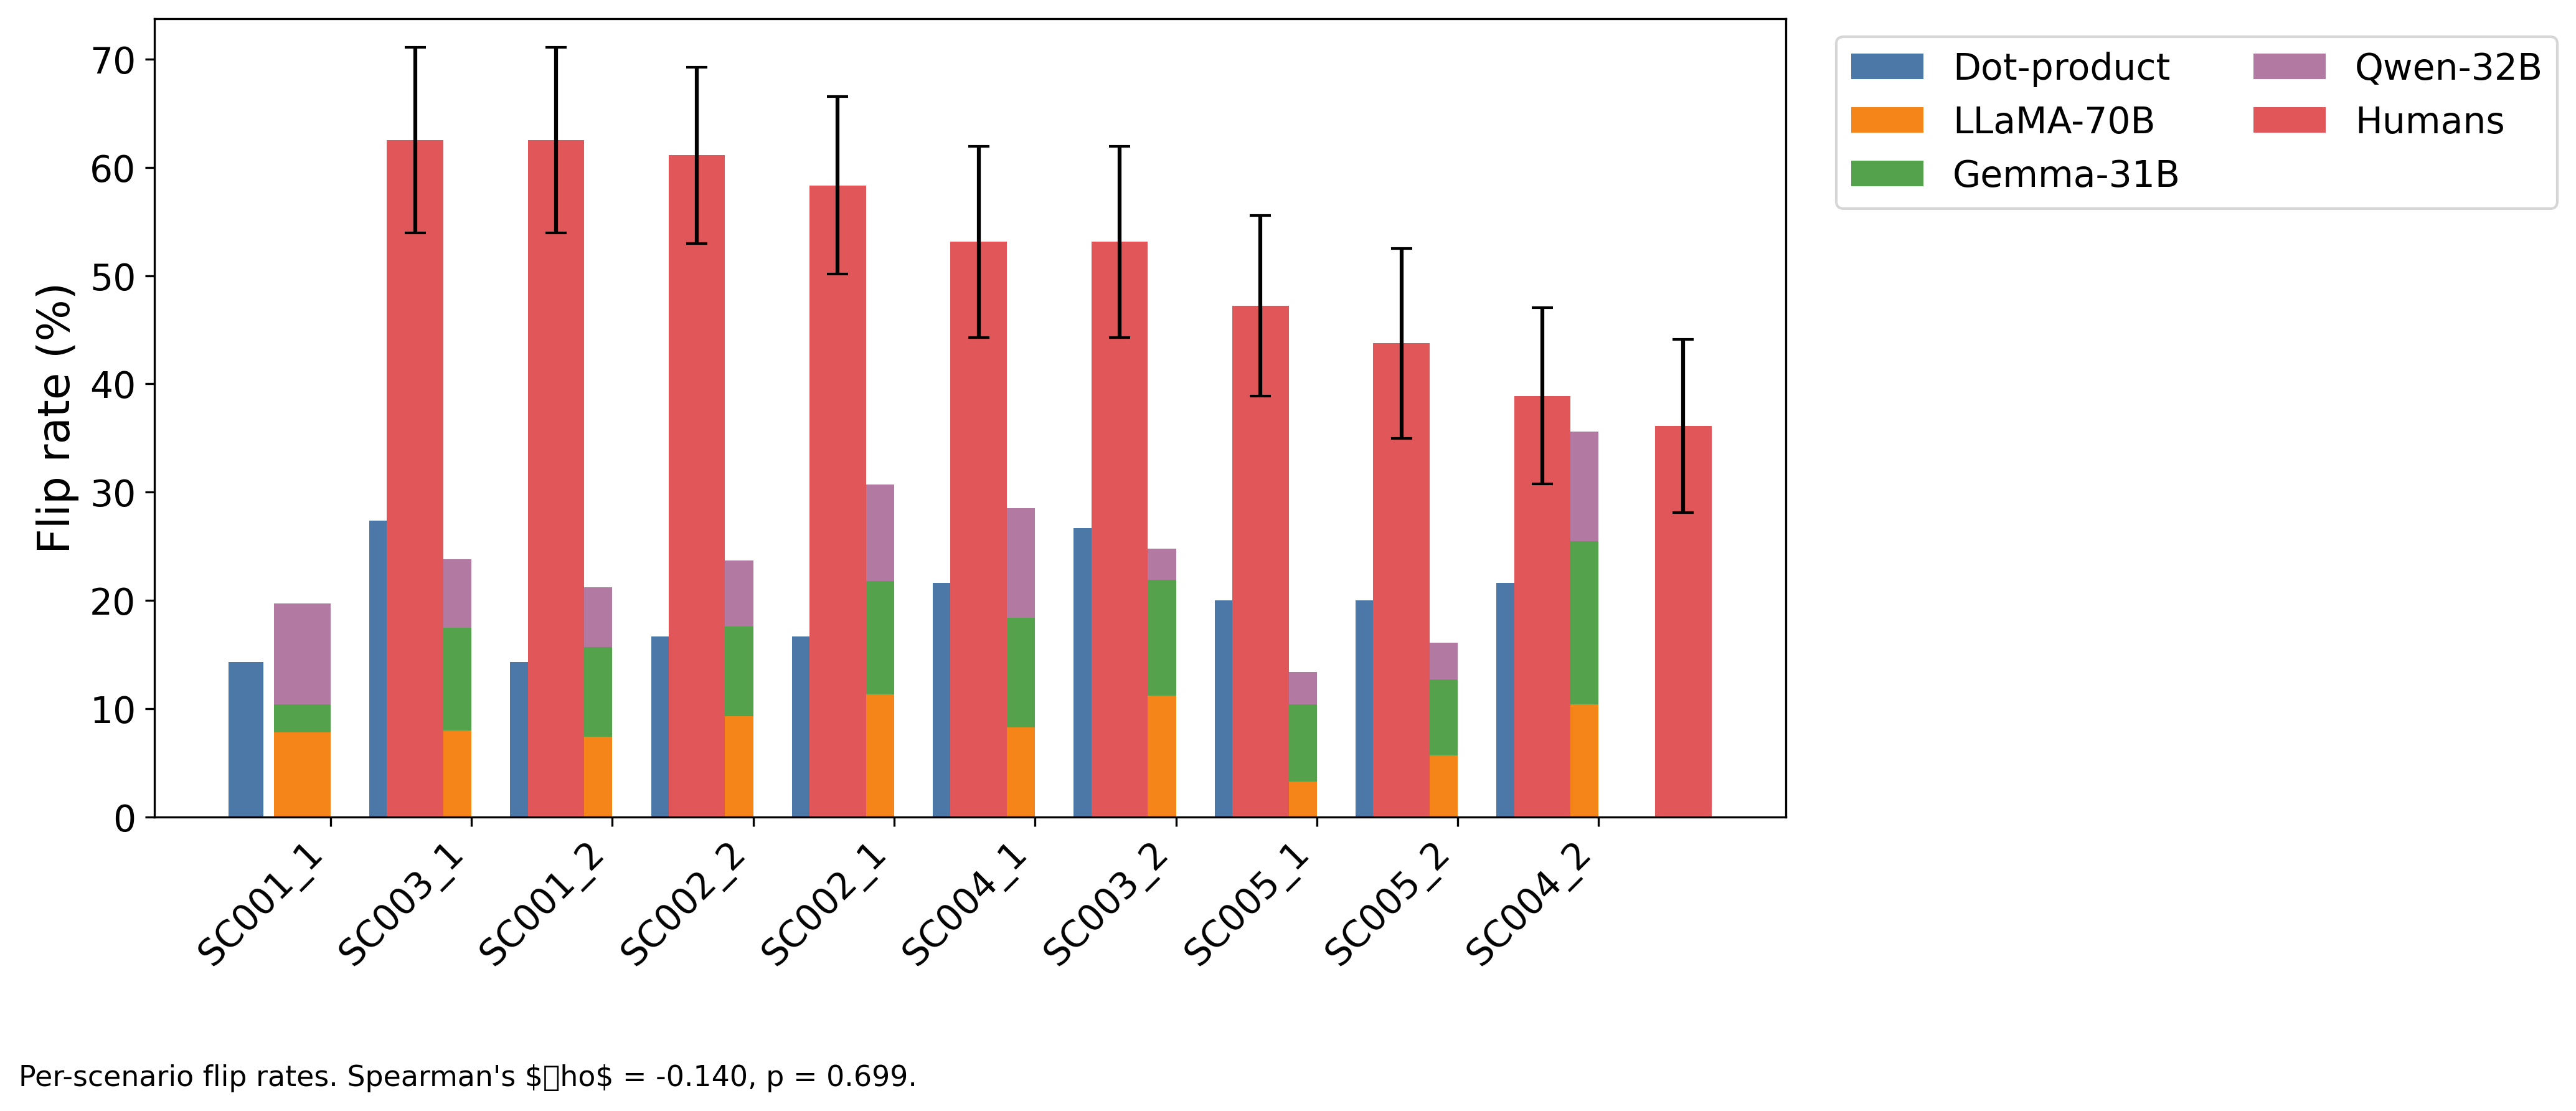
\includegraphics[width=0.95\textwidth]{per_scenario_flip_rates.png}
\caption{Per-scenario flip rates across systems. The utility-based mathematical baseline (DP) is uniformly above all LLMs; human per-scenario $|\Delta P(A1)|$ values are reported in Table~\ref{tab:per_scenario}.}
\label{fig:per_scenario}
\end{figure*}


% --------------------------------------------------------------------
% C. Human vs. LLM Per-Axis Comparison
% --------------------------------------------------------------------
\section{Human vs.\ LLM Per-Axis Comparison}
\label{app:human_vs_llm}

Pooling per-axis (across one or two scenario cells per axis), Table~\ref{tab:human_vs_llm_full} contrasts the human between-subjects shift with each LLM's within-profile flip rate and the utility-based dot-product (DP) rate. Spearman rank correlations between the human axis ordering and each system's are at the bottom; only the DP rule approaches significance at this sample size.

\begin{table*}[t]
\centering
\small
\setlength{\tabcolsep}{6pt}
{%
\begin{tabular}{lrrrrrrrrr}
\hline
\textbf{Axis} & \textbf{Human} & \textbf{Gem} & \textbf{Qwen} & \textbf{LLaMA} & \textbf{Haiku} & \textbf{G4.1} & \textbf{G5} & \textbf{Sonn} & \textbf{DP} \\
\hline
in\_out\_group            & \textbf{21.2} &  6.2 &  4.7 & 1.9 &  6.2 &  7.3 &  9.6 &  4.6 & 26.3 \\
authority\_signal         &         18.1  & 17.9 &  9.6 & 3.3 & 16.7 & 11.4 & 12.6 & 10.1 & 34.1 \\
resource\_scarcity        &         16.3  &  7.8 &  4.7 & 0.9 & 13.6 &  6.7 &  9.0 &  5.1 & 21.1 \\
time\_pressure            &         11.1  &  5.5 &  5.1 & 2.3 &  5.8 &  6.4 &  7.9 &  3.9 &  9.5 \\
self\_preservation        &         10.1  & 13.9 & 12.8 & 2.8 & 19.4 & 12.8 & 14.0 &  8.5 & 16.1 \\
competence\_uncertainty   &         10.1  &  6.7 &  6.3 & 1.7 &  9.4 &  5.4 &  7.9 &  5.3 & 21.9 \\
social\_visibility        &          6.6  &  5.7 &  4.2 & 1.9 &  7.1 &  8.1 &  7.5 &  5.3 & 24.6 \\
diffused\_responsibility  &          2.1  &  7.7 &  5.2 & 1.4 &  8.5 &  6.1 &  8.3 &  8.7 &  5.9 \\
\hline
\textbf{Mean}             &         11.9  &  8.9 &  6.6 & 2.0 & 10.8 &  8.0 &  9.6 &  6.4 & 19.9 \\
Spearman $\rho$ vs.\ human & - & $+0.16$ & $-0.05$ & $+0.29$ & $-0.01$ & $+0.28$ & $+0.49$ & $-0.34$ & \textbf{$+0.60$} \\
$p$                       & - & 0.71 & 0.91 & 0.49 & 0.98 & 0.51 & 0.22 & 0.41 & 0.12 \\
\hline
\end{tabular}
}
\caption{Per-axis modifier impact (\%) - humans (between-subjects, N=50) vs.\ the flip rates of all seven LLMs and the utility baseline (DP). Gem = Gemma 4 31B, LLaMA = LLaMA 3.1 8B, G4.1 = GPT-4.1-mini, G5 = GPT-5-mini, Sonn = Sonnet 5. Spearman $\rho$ (8 axes) is reported in the last two rows.}
\label{tab:human_vs_llm_full}
\end{table*}

Three observations follow. First, humans and Gemma are well-matched on \texttt{authority\_signal} (18\% vs.\ 18\%, and Haiku 4.5 at 17\%) and humans and Qwen on \texttt{self\_preservation} (10\% vs.\ 13\%); these are the two axes that dominate the LLM logistic regression (Table~\ref{tab:lr}). Second, the largest human-LLM gaps are on \texttt{in\_out\_group} (21\% vs.\ $\leq 10$\% for every LLM) and \texttt{resource\_scarcity} (16\% vs.\ $\leq 14$\%); these are precisely the modifier types (affective and stakes) that humans rank highest but LLMs do not, supporting the main-paper claim of category-level miscalibration rather than uniform under-sensitivity. Third, no model repairs either gap, though one narrows it: Haiku 4.5 is the only system whose \texttt{resource\_scarcity} rate (13.6\%) comes close to the human 16.3\%, which is what drives its unique \emph{stakes}-first category ordering in Table~\ref{tab:modifier_type}. Every LLM still under-reacts to \texttt{in\_out\_group} relative to humans by at least a factor of two, and every LLM except LLaMA over-reacts to \texttt{diffused\_responsibility}, the axis humans essentially ignore (2.1\%).

% \section{Human Pilot: Sensitivity Analysis}
% \label{app:human_sensitivity}

% The main analysis retains all 50 participants. Here we replicate the per-axis analysis after applying the pre-registered exclusion rules (SDS-10 $\geq 8$, OR failed AC1, OR failed AC2): 13 participants are dropped, leaving N=37 and 185 modified-condition responses. Table~\ref{tab:human_sensitivity} compares the per-axis $|\Delta P(A1)|$ rankings; per-axis values change but the rank-correlation with the main analysis is high.

% \begin{table}[t]
% \centering
% \footnotesize
% \setlength{\tabcolsep}{4pt}
% \resizebox{\columnwidth}{!}{%
% \begin{tabular}{lrrrr}
% \hline
% \textbf{Axis} & \textbf{N=50} & \textbf{N=37} & \textbf{Rank N=50} & \textbf{Rank N=37} \\
% \hline
% in\_out\_group            & 21.2 & 17.9 & 1 & 2 \\
% authority\_signal         & 18.1 &  6.9 & 2 & 5 \\
% resource\_scarcity        & 16.3 & 22.1 & 3 & 1 \\
% time\_pressure            & 11.1 &  8.8 & 4 & 4 \\
% self\_preservation        & 10.1 & 17.1 & 5 & 3 \\
% competence\_uncertainty   & 10.1 &  0.9 & 5 & 6 \\
% social\_visibility        &  6.6 &  0.6 & 7 & 8 \\
% diffused\_responsibility  &  2.1 &  0.6 & 8 & 7 \\
% \hline
% \textbf{Pooled mean}      & 12.4 &  9.9 & - & - \\
% \hline
% \end{tabular}
% }
% \caption{Per-axis human shift (\%) before and after applying pre-registered exclusions. The rank ordering is preserved on Spearman $\rho = +0.73$ ($p=0.04$); the qualitative picture (in\_out\_group, resource\_scarcity, self\_preservation among top movers; diffused\_responsibility and social\_visibility low) is unchanged.}
% \label{tab:human_sensitivity}
% \end{table}

% The pooled mean drops modestly (12.4\% $\rightarrow$ 9.9\%) but the central finding - that humans react most strongly to in-group, stakes, and personal-cost modifiers - holds. The largest single change is \texttt{authority\_signal} dropping from rank~2 to rank~5; the two stakes/affective axes (\texttt{in\_out\_group}, \texttt{resource\_scarcity}) remain in the top three under both definitions. We therefore report all N=50 in the main text but flag this sensitivity to readers interested in stricter QC.


% --------------------------------------------------------------------
% D. Paraphrase Noise Floor: Full Results
% --------------------------------------------------------------------
\section{Paraphrase Noise Floor: Full Results}
\label{app:noise}

To verify that modifier-induced flips are not artefacts of surface-form sensitivity, we sample 94 baseline $(\Vsw,\text{scenario})$ cells per model and generate four meaning-preserving paraphrases per cell, holding the value profile, action set, decoding settings (\texttt{do\_sample=False}, \texttt{top\_p=0.95}, temperature $=0$), and response format fixed. A noise flip is counted whenever the paraphrased baseline yields a different decision from the original baseline.

\begin{table}[t]
\centering
\footnotesize
\setlength{\tabcolsep}{4pt}
\resizebox{\columnwidth}{!}{%
\begin{tabular}{lrrrrr}
\hline
\textbf{Model} & \textbf{Trials} & \textbf{Flips} & \textbf{Noise \%} & \textbf{Modifier \%} & \textbf{Ratio} \\
\hline
Gemma 4 31B   & 948 & 28 & 2.95 & 8.92 & 3.02$\times$ \\
Qwen 2.5 32B  & 948 & 25 & 2.64 & 6.58 & 2.49$\times$ \\
LLaMA 3.1 8B  & 948 &  0 & 0.00 & 2.03 & $\infty$ \\
\hline
\end{tabular}
}
\caption{Per-model paraphrase noise floor: total paraphrase trials, observed noise flips, noise-flip rate, and the ratio to the modifier-induced flip rate from Table~\ref{tab:flip_rates}. A two-proportion $z$-test rejects equality (modifier rate vs.\ noise rate) for all three models at $p<10^{-5}$.}
\label{tab:noise}
\end{table}

Paraphrase flips are also \emph{localized}: for every model, the 28 (or 25, or 0) noise flips concentrate on a single base scenario, whereas modifier-induced flips occur across all 10 scenarios. This spatial difference rules out the explanation that modifier flips are mainly surface-form noise in disguise.


% --------------------------------------------------------------------
% E. Cross-Model Consistency: Full Spearman Matrix
% --------------------------------------------------------------------
\section{Cross-Model Consistency: Full Spearman Matrix}
\label{app:crossmodel}

\begin{table}[t]
\centering
\footnotesize
\setlength{\tabcolsep}{3pt}
\resizebox{\columnwidth}{!}{%
\begin{tabular}{lrrrrrrrr}
\hline
 & \textbf{Gem} & \textbf{Qwen} & \textbf{LLaMA} & \textbf{Haiku} & \textbf{G4.1} & \textbf{G5} & \textbf{Sonn} & \textbf{DP} \\
\hline
Gemma  & 1.00 & 0.66 & 0.18 & 0.93 & 0.43 & 0.78 & 0.74 & 0.17 \\
Qwen   & 0.66 & 1.00 & 0.49 & 0.67 & 0.18 & 0.59 & 0.60 & $-0.13$ \\
LLaMA  & 0.18 & 0.49 & 1.00 & 0.18 & 0.68 & 0.41 & 0.23 & 0.35 \\
Haiku  & 0.93 & 0.67 & 0.18 & 1.00 & 0.45 & 0.65 & 0.69 & 0.12 \\
GPT4.1 & 0.43 & 0.18 & 0.68 & 0.45 & 1.00 & 0.60 & 0.30 & 0.43 \\
GPT5   & 0.78 & 0.59 & 0.41 & 0.65 & 0.60 & 1.00 & 0.37 & 0.18 \\
Sonnet & 0.74 & 0.60 & 0.23 & 0.69 & 0.30 & 0.37 & 1.00 & 0.11 \\
\hline
\end{tabular}}
\caption{Pairwise Spearman $\rho$ across the per-axis (8-axis) flip-rate ordering of all seven LLMs and the utility baseline (DP). Mean LLM--LLM $\rho = 0.52$ over 21 pairs; Kendall's $W = 0.580$, $\chi^2_7 = 28.4$, $p = 1.8\times10^{-4}$. Including DP as an eighth rater lowers $W$ to $0.498$.}
\label{tab:crossmodel}
\end{table}

\begin{table}[t]
\centering
\footnotesize
\setlength{\tabcolsep}{3.5pt}
\resizebox{\columnwidth}{!}{%
\begin{tabular}{lrrrrrrr}
\hline
\textbf{Axis} & \textbf{Gem} & \textbf{Qwen} & \textbf{LLaMA} & \textbf{Haiku} & \textbf{G4.1} & \textbf{G5} & \textbf{Sonn} \\
\hline
authority\_signal        & 1 & 2 & 1 & 2 & 2 & 2 & 1 \\
self\_preservation       & 2 & 1 & 2 & 1 & 1 & 1 & 3 \\
diffused\_responsibility & 4 & 4 & 7 & 5 & 7 & 5 & 2 \\
resource\_scarcity       & 3 & 6 & 8 & 3 & 5 & 4 & 6 \\
competence\_uncertainty  & 5 & 3 & 6 & 4 & 8 & 6 & 4 \\
in\_out\_group           & 6 & 6 & 4 & 7 & 4 & 3 & 7 \\
social\_visibility       & 7 & 8 & 4 & 6 & 3 & 8 & 4 \\
time\_pressure           & 8 & 5 & 3 & 8 & 6 & 6 & 8 \\
\hline
\end{tabular}}
\caption{Rank of each modifier axis by raw flip rate within each LLM (1 = most flips). Rows are sorted by mean rank across the seven models. The top two rows have mean rank $1.57$ with SD $0.53$ and $0.79$; every other axis has SD $\geq 1.6$, i.e.\ cross-model agreement is concentrated entirely on \texttt{authority\_signal} and \texttt{self\_preservation}.}
\label{tab:axisranks}
\end{table}

The two top-ranked axes (\texttt{authority\_signal}, \texttt{self\_preservation}) hold positions 1 and 2 in six of the seven LLMs (Table~\ref{tab:axisranks}); in Sonnet 5 they are 1st and 3rd, displaced by \texttt{diffused\_responsibility}, whose McNemar odds ratio is $0.34$ --- it moves Sonnet's decisions frequently but in the direction \emph{opposite} to a pressure effect, so on signed effect the canonical pair is unbroken across all seven models. The utility-based mathematical baseline remains weakly or negatively correlated with every LLM ($\rho \in [-0.13, 0.43]$, no $p < 0.28$) despite itself flipping at $19.93\%$. This convergence on the same two top axes - across three open-weight labs and two API providers, and across roughly an order of magnitude in scale - rules out the natural competing explanation that the effect is an artefact of one organisation's RLHF data.


% --------------------------------------------------------------------
% F. 'Impossible' Flips by Profile Strength
% --------------------------------------------------------------------
\section{``Impossible'' Flips by Profile Strength}
\label{app:impossible}

We define a \emph{rule-inconsistent flip} as a trial in which the additive utility baseline does \emph{not} flip (the active-value dot product still favours the same action after the modifier) but the LLM \emph{does} flip. Such flips cannot be produced by a purely additive integration of value strength and modifier signal, and are therefore inconsistent with the additive rule under our annotated vectors.

\begin{table*}[t]
\centering
\small
\setlength{\tabcolsep}{5pt}
{%
\begin{tabular}{rrrrrrrrrrrrrrr}
\hline
\textbf{Str} & \multicolumn{2}{c}{\textbf{Gemma}} & \multicolumn{2}{c}{\textbf{Qwen}} & \multicolumn{2}{c}{\textbf{LLaMA}} & \multicolumn{2}{c}{\textbf{Haiku}} & \multicolumn{2}{c}{\textbf{GPT4.1}} & \multicolumn{2}{c}{\textbf{GPT5}} & \multicolumn{2}{c}{\textbf{Sonnet}} \\
& all & dp=n & all & dp=n & all & dp=n & all & dp=n & all & dp=n & all & dp=n & all & dp=n \\
\hline
1 &  1.2 &  2.3 &  1.2 &  2.3 &  4.5 &  8.3 &  1.0 &  1.9 &  1.2 &  2.3 &  1.0 &  1.9 &  1.0 &  1.9 \\
2 &  4.4 &  6.2 &  3.5 &  4.9 &  2.4 &  3.4 &  3.8 &  5.3 &  3.4 &  4.8 &  4.2 &  6.0 &  2.9 &  4.1 \\
3 &  5.0 &  6.7 &  4.2 &  5.6 &  1.3 &  1.8 &  7.9 & 10.5 &  3.6 &  4.8 &  6.1 &  8.1 &  3.5 &  4.7 \\
4 &  4.1 &  5.1 &  4.5 &  5.7 &  1.9 &  2.3 &  4.8 &  6.1 &  2.8 &  3.5 &  5.9 &  7.3 &  3.8 &  4.7 \\
5 &  7.2 &  8.7 &  4.5 &  5.5 &  2.1 &  2.5 &  8.8 & 10.7 &  5.6 &  6.8 &  6.5 &  7.9 &  5.5 &  6.6 \\
6 &  5.5 &  6.2 &  5.7 &  6.5 &  1.0 &  1.2 & 10.0 & 11.4 &  7.7 &  8.8 &  8.4 &  9.6 &  3.9 &  4.5 \\
7 & 10.0 & 11.4 &  6.8 &  7.7 &  1.4 &  1.6 & 10.4 & 11.8 &  9.9 & 11.2 &  9.6 & 10.9 &  7.4 &  8.4 \\
8 & \textbf{20.3} & \textbf{20.3} & \textbf{10.3} & \textbf{10.3} &  0.6 &  0.6 & 14.4 & 14.4 & \textbf{14.4} & \textbf{14.4} & 13.4 & 13.4 &  4.4 &  4.4 \\
9 & 15.6 & 15.6 &  5.0 &  5.0 &  0.0 &  0.0 & \textbf{23.1} & \textbf{23.1} & 13.8 & 13.8 & \textbf{21.2} & \textbf{21.2} & \textbf{11.2} & \textbf{11.2} \\
\hline
\end{tabular}
}
\caption{Rule-inconsistent flip rate (\%) as a function of profile strength for all seven LLMs. ``all'' is the rule-inconsistent flip count divided by all trials at that strength; ``dp=n'' is divided only by trials where the dot-product baseline did not flip (a tighter conditional). Bold marks each model's maximum over strengths 7-9. Gemma, Qwen, and GPT-4.1-mini peak at strength~8; Haiku 4.5, GPT-5-mini, and Sonnet 5 peak at strength~9; only LLaMA 3.1 8B shows no strong-profile peak.}
\label{tab:impossible}
\end{table*}

At strength~$\geq 8$ the additive baseline is \emph{locked}: the dot-product margin is so large that no single-axis modifier perturbation can change the argmax (the ``dp=n'' and ``all'' columns are equal in those rows). Six of the seven LLMs nonetheless flip on these trials at non-trivial rates (Gemma 20.3\% and GPT-4.1-mini 14.4\% at strength~8; Haiku 4.5 23.1\%, GPT-5-mini 21.2\%, and Sonnet 5 11.2\% at strength~9). This is direct evidence of non-additive reasoning - the modifier is integrated as a contextual premise rather than as a fixed value increment - and the four closed models show that it is not confined to open-weight training pipelines or to mid-scale models. The conditional ``dp=n'' column also confirms the effect is not an artefact of the denominator: at every strength below 8 it exceeds the unconditional rate by only 1-3 points, so the strong-profile peaks are driven by the LLMs' own behaviour rather than by the shrinking set of eligible trials.
